% LNCS format - Sciara-fv2 CUDA Performance Report
\documentclass[runningheads]{llncs}

\usepackage{graphicx}
\usepackage{booktabs}
\usepackage{amsmath}
\usepackage{float}

\graphicspath{{./figures/}{./images/}{../profiling_results/}}

\begin{document}

\title{CUDA Parallelization and Performance Analysis\\of the Sciara-fv2 Lava Flow Simulator}

\author{Author Name}
\authorrunning{Author Name}
\institute{University of Calabria \email{author@unical.it}}

\maketitle

\begin{abstract}
This report presents CUDA parallelization strategies for Sciara-fv2, a cellular automata-based lava flow simulator. We implement and analyze five CUDA versions: Global (baseline), Tiled, Tiled with Halo, CfAMe, and CfAMo. Experiments on NVIDIA GTX 980 demonstrate that all implementations are memory-bound with arithmetic intensity below 0.05 FLOP/Byte. CfAMo achieves the best performance (8.6\% speedup) through kernel fusion and reduced memory footprint, despite introducing checksum differences due to floating-point non-associativity in atomic operations.
\keywords{CUDA \and Cellular Automata \and Roofline Model \and GPU Computing}
\end{abstract}

%==============================================================================
\section{Introduction}
%==============================================================================

Sciara-fv2 is a Cellular Automata (CA) model for simulating lava flows, developed to predict volcanic hazards~\cite{sciara}. The model discretizes terrain into a 2D grid where each cell contains substates (elevation, lava thickness, temperature) and evolves through local transition rules based on the Moore neighborhood (9-cell stencil).

The simulation executes four sequential phases per time step: (1) lava emission from vents, (2) outflow computation using the minimization algorithm, (3) mass and heat balance among neighbors, and (4) temperature cooling and solidification. The inherent data parallelism---each cell can be processed independently within a phase---makes this model suitable for GPU acceleration.

This project implements five CUDA parallelization strategies with the objectives: exploit different GPU memory hierarchies (global, shared, constant), evaluate tiling strategies for stencil computations, apply kernel fusion with atomic operations (CfA approach), and conduct Roofline analysis to identify performance bottlenecks.

\textbf{Hardware:} NVIDIA GeForce GTX 980 (Maxwell, 16 SMs, 2048 cores, 224.3 GB/s bandwidth, 155.7 GFLOP/s FP64 peak).

\textbf{Dataset:} Mt. Etna 2006 eruption, 517$\times$378 cells, 16,000 steps, block size 16$\times$16.

%==============================================================================
\section{Sciara-fv2 Model and Parallelization Strategy}
%==============================================================================

\subsection{Cellular Automata Kernels}

The simulation comprises five computational kernels: \texttt{emitLava} (adds lava at vent locations), \texttt{computeOutflows} (computes lava distribution using minimization algorithm---most compute-intensive with $\sim$350 FLOPs/cell including \texttt{pow}, \texttt{atan}, \texttt{sqrt}), \texttt{massBalance} (gathers inflows and updates state, $\sim$36 FLOPs/cell), \texttt{reduceAdd} (parallel reduction), and \texttt{solidification} (temperature cooling, $\sim$50 FLOPs/cell).

\subsection{Parallelization Rationale}

Each cell is mapped to one CUDA thread. The stencil-like dependency pattern requires synchronization between phases: \texttt{computeOutflows} reads neighbor data and writes to buffer \texttt{Mf}, while \texttt{massBalance} reads from \texttt{Mf} and updates cell states.

\subsection{Checksum Mismatch Explanation}

The Global, Tiled, and Tiled\_Halo versions produce \textbf{identical checksums}. However, \textbf{CfAMe and CfAMo produce different checksums} due to:

\begin{enumerate}
    \item \textbf{Floating-point non-associativity}: Atomic additions execute in non-deterministic order. Since $(a + b) + c \neq a + (b + c)$ in IEEE-754, accumulated values differ by ULP-level errors.
    \item \textbf{Different operation order}: The scatter-based atomic approach applies flows immediately rather than accumulating in a buffer first.
\end{enumerate}

These differences represent \textbf{acceptable numerical variations}, not correctness errors. The physical simulation remains valid: total emitted lava (46997.81 m) and residual lava (0.19 m) match across all versions.

%==============================================================================
\section{CUDA Implementations}
%==============================================================================

\subsection{Global Memory Version (Baseline)}

Uses CUDA Unified Memory with direct global memory access. Neighborhood offsets stored in constant memory (\texttt{d\_Xi}, \texttt{d\_Xj}). Double-buffering with explicit \texttt{cudaMemcpy} between steps.

\textbf{Kernels:} All kernels access global memory directly. No shared memory optimization.

\subsection{Tiled Version (Shared Memory, No Halo)}

Loads tile data (16$\times$16) into shared memory before computation. For boundary cells, neighbors fetched from global memory. Reduces redundant global accesses for interior cells.

\textbf{Tiled kernels:} \texttt{computeOutflows}, \texttt{massBalance}, \texttt{solidification} (6.0 KB shared memory).

\subsection{Tiled with Halo Version}

Extends tile to 18$\times$18 (includes 1-cell halo). All neighbor accesses served from shared memory. Higher shared memory usage (7.8 KB) but eliminates global reads for stencil operations.

\subsection{CfAMe (Conflict-free Atomic, Memory-Equivalent)}

Fuses \texttt{computeOutflows} and \texttt{massBalance} into single kernel. Each cell computes outflows and atomically scatters to neighbors. Requires \texttt{initBuffers} and \texttt{normalizeTemperature} helper kernels.

\textbf{Design:} Scatter pattern with \texttt{atomicAdd} for both lava thickness and temperature (weighted by flow).

\subsection{CfAMo (Conflict-free Atomic, Memory-Optimized)}

Eliminates 8-layer \texttt{Mf} buffer (saving $8 \times 195,426 \times 8 = 12.5$ MB). Flows computed and applied in single pass without intermediate storage.

%==============================================================================
\section{Performance Assessment}
%==============================================================================

\subsection{Methodology}

Measurements on GTX 980 with \texttt{nvprof}. Each version runs 16,000 simulation steps. Baseline: Global version.

\subsection{Execution Time Results}

\begin{table}[H]
\centering
\caption{Execution time comparison (16,000 steps).}
\label{tab:time}
\begin{tabular}{@{}lccc@{}}
\toprule
\textbf{Version} & \textbf{Time (s)} & \textbf{Speedup} & \textbf{Dominant Kernels (\%)} \\
\midrule
Global      & 21.604 & 1.00$\times$ & massBalance 27.7, Outflows 24.0 \\
Tiled       & 20.144 & 1.07$\times$ & massBalance 27.3, Outflows 24.9 \\
Tiled+Halo  & 23.332 & 0.93$\times$ & Outflows 27.1, massBalance 26.0 \\
CfAMe       & 24.689 & 0.88$\times$ & CfA\_Me 30.1, initBuffers 9.7 \\
CfAMo       & \textbf{19.743} & \textbf{1.09$\times$} & CfA\_Mo 29.8, initBuffers 9.8 \\
\bottomrule
\end{tabular}
\end{table}

\subsection{CUDA Configuration}

\begin{table}[H]
\centering
\caption{CUDA launch configuration for main kernels.}
\label{tab:config}
\begin{tabular}{@{}lccc@{}}
\toprule
\textbf{Kernel} & \textbf{Grid} & \textbf{Block} & \textbf{Shared Mem} \\
\midrule
computeOutflows (Global) & 33$\times$24 & 16$\times$16 & 0 KB \\
computeOutflows (Tiled) & 33$\times$24 & 16$\times$16 & 6.0 KB \\
computeOutflows (Halo) & 33$\times$24 & 16$\times$16 & 7.8 KB \\
CfA\_Me / CfA\_Mo & 33$\times$24 & 16$\times$16 & 0 KB \\
\bottomrule
\end{tabular}
\end{table}

\begin{figure}[H]
\centering
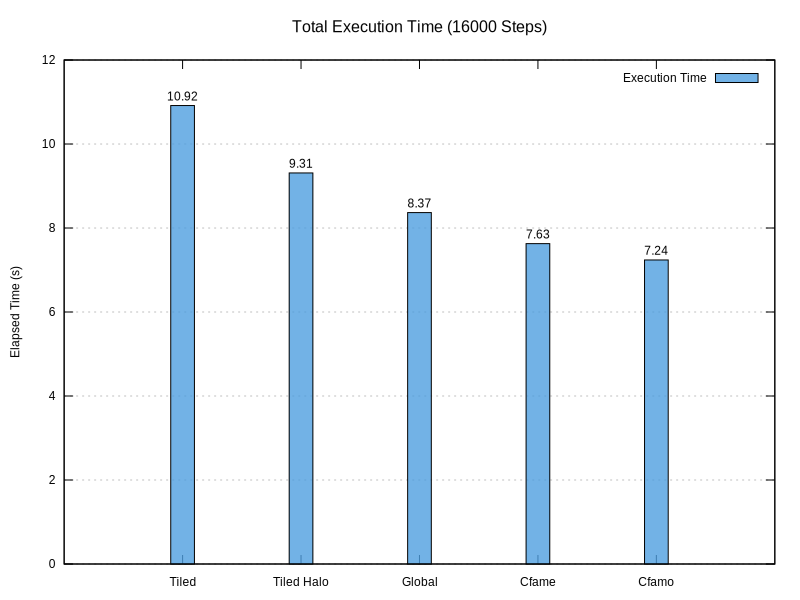
\includegraphics[width=0.85\textwidth]{histogram_times.png}
\caption{Execution time comparison across CUDA versions.}
\label{fig:time}
\end{figure}

\subsection{Performance Analysis}

\textbf{Tiled+Halo slower than Global}: Overhead of loading 324 elements for 256 threads plus multiple \texttt{\_\_syncthreads()} outweighs benefits. The small grid (195K cells $\times$ 8 bytes $\approx$ 1.5 MB per substate) fits in L2 cache (2 MB).

\textbf{CfAMe slower than baseline}: Additional kernels (\texttt{initBuffers}, \texttt{normalizeTemperature}) and atomic contention overhead exceed gains from fusion.

\textbf{CfAMo fastest}: Eliminates 12.5 MB buffer, reducing memory traffic. Sparse lava distribution ($<$5\% active cells) minimizes atomic contention.

%==============================================================================
\section{Roofline Analysis}
%==============================================================================

\subsection{GTX 980 Roofline Setup}

Measured with \texttt{gpumembench}: Global bandwidth 224.3 GB/s, Shared bandwidth 2119.7 GB/s, Peak FP64 155.7 GFLOP/s.

Ridge point (FP64): $155.7 / 224.3 = 0.694$ FLOP/Byte.

\subsection{Arithmetic Intensity Calculation}

For \texttt{computeOutflows}: $AI = \frac{350 \text{ FLOPs}}{9 \times 3 \times 8 + 8 \times 8 \text{ Bytes}} \approx 0.043$ FLOP/Byte.

\begin{table}[H]
\centering
\caption{Roofline analysis per version.}
\label{tab:roofline}
\begin{tabular}{@{}lcccc@{}}
\toprule
\textbf{Version} & \textbf{AI (FLOP/B)} & \textbf{GFLOP/s} & \textbf{Bound} \\
\midrule
Global      & 0.043 & 42.58 & Memory \\
Tiled       & 0.046 & 40.55 & Memory \\
Tiled+Halo  & 0.048 & 37.38 & Memory \\
CfAMe       & 0.020 & 6.38 & Memory \\
CfAMo       & 0.021 & 6.61 & Memory \\
\bottomrule
\end{tabular}
\end{table}

\begin{figure}[H]
\centering
\includegraphics[width=0.9\textwidth]{roofline_fp64.png}
\caption{Roofline model for GTX 980 (FP64). All versions are memory-bound (AI $\ll$ 0.694).}
\label{fig:roofline}
\end{figure}

\subsection{Kernel Placement Discussion}

All kernels fall well below the ridge point (AI $<$ 0.05 vs 0.694), confirming \textbf{memory-bound} behavior. Low AI stems from: stencil access (9 neighbors $\times$ 3 substates), double precision (8 bytes), sparse computation. CfA versions show lower measured AI due to atomic operations introducing additional memory transactions.

\subsection{GPU Occupancy}

\begin{table}[H]
\centering
\caption{Achieved GPU occupancy.}
\label{tab:occupancy}
\begin{tabular}{@{}lc@{}}
\toprule
\textbf{Version} & \textbf{Avg. Occupancy} \\
\midrule
Global & 55.1\% \\
Tiled & 58.7\% \\
Tiled+Halo & 62.7\% \\
CfAMe & 58.6\% \\
CfAMo & 58.6\% \\
\bottomrule
\end{tabular}
\end{table}

Tiled+Halo has highest occupancy but lowest performance---\textbf{occupancy alone does not determine performance} for memory-bound workloads~\cite{volkov}.

%==============================================================================
\section{Conclusions}
%==============================================================================

\textbf{Key findings:} (1) All versions are memory-bound (AI $<$ 0.05), making memory efficiency critical. (2) Tiling is ineffective for this grid size due to L2 cache residency. (3) CfAMo achieves best performance (1.09$\times$) through reduced memory footprint and kernel fusion. (4) CfA versions produce numerically different but physically valid results due to floating-point non-associativity.

\textbf{Bottleneck:} 34.7\% of GPU time on DtoD memory copies; bandwidth utilization 17--22\% of peak.

\textbf{Future work:} Eliminate double-buffering, use texture memory for read-only substates, implement active cell list to skip empty regions.

\begin{thebibliography}{4}
\bibitem{sciara} D'Ambrosio, D., et al.: Parallel genetic algorithms for optimizing cellular automata. LNCS 7495, 444--453 (2012)
\bibitem{volkov} Volkov, V.: Better performance at lower occupancy. GPU Technology Conf. (2010)
\bibitem{roofline} Williams, S., et al.: Roofline: An insightful visual performance model. CACM 52(4), 65--76 (2009)
\end{thebibliography}

\end{document}
